% Small AI Academic Paper Sample using LaTeX + BibTeX
\documentclass[11pt]{article}

% Packages
\usepackage[a4paper,margin=1in]{geometry}
\usepackage{times}
\usepackage{microtype}
\usepackage{hyperref}
\usepackage{graphicx}
% Search for images: legacy figures/, new manual_data/ and generated_data/ (and fallback absolute path from repo root)
\graphicspath{{generated_data/}{manual_data/}{figures/}{src/latex/generated_data/}{src/latex/manual_data/}{src/latex/figures/}}
\usepackage{booktabs}
\usepackage{amsmath, amssymb}
\usepackage{xcolor}
\usepackage[numbers]{natbib}

% Hyperref setup
\hypersetup{
  colorlinks=true,
  linkcolor=blue,
  citecolor=teal,
  urlcolor=magenta,
  pdftitle={Small AI Paper Sample},
  pdfauthor={Your Name},
}

% Title
\title{A Small Sample Paper in Artificial Intelligence}
\author{Your Name \\ Your Affiliation \\ \texttt{you@example.com}}
\date{September 16, 2025}

\begin{document}
\maketitle

\begin{abstract}
We provide a compact LaTeX template for an AI research paper with Bib\TeX{} references and common sections. It includes figures, tables, and sample citations to classic and modern works in machine learning and natural language processing.
\end{abstract}

% Auto-generated figure from src/python will be saved under src/latex/generated_data/simple_plot.png
% See README for how to regenerate.
\begin{figure}[t]
  \centering
  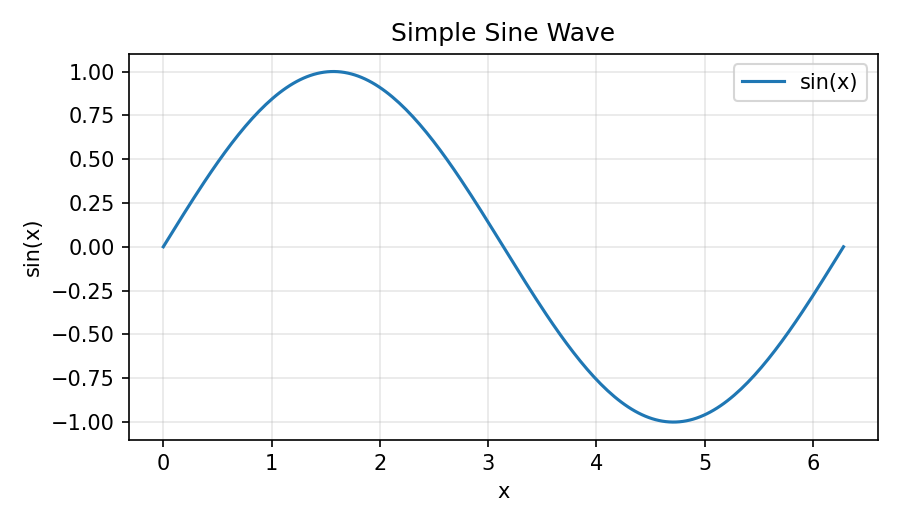
\includegraphics[width=0.65\linewidth]{simple_plot.png}
  \caption{A simple plot generated by the Python helper.}
  \label{fig:simple}
\end{figure}

% Example of a manually supplied image placed under manual_data/
\begin{figure}[t]
  \centering
  
\includegraphics[width=0.5\linewidth]{manual_placeholder.png}
  \caption{An example manually curated image. Replace this placeholder with your own asset.}
  \label{fig:manual}
\end{figure}

\section{Introduction}
Artificial Intelligence (AI) has progressed rapidly from early symbolic systems to modern deep learning and large language models. Foundational algorithms such as the perceptron~\citep{rosenblatt1958perceptron} and backpropagation~\citep{rumelhart1986learning} paved the way for convolutional networks~\citep{lecun1998gradient,krizhevsky2012imagenet} and attention-based architectures~\citep{vaswani2017attention,devlin2018bert,brown2020language}.

This sample paper demonstrates a minimal LaTeX setup using Bib\TeX{} for citations, section includes, and typical assets like figures and tables. It is intentionally small so you can adapt it quickly for your own AI projects.

\section{Related Work}
Classical neural network training relies on gradient-based optimization~\citep{rumelhart1986learning}. Convolutional architectures dominated vision benchmarks beginning with LeNet~\citep{lecun1998gradient} and surged after ImageNet results by AlexNet~\citep{krizhevsky2012imagenet}. In NLP, recurrent architectures gave way to self-attention models, culminating in the Transformer~\citep{vaswani2017attention}, BERT~\citep{devlin2018bert}, and large autoregressive models~\citep{brown2020language}.

Surveys and textbooks provide broader context, but here we keep the scope concise and refer readers to the cited works for details.

\section{Method}
We outline a generic supervised learning setup. Given a dataset of input--label pairs $\{(x_i, y_i)\}_{i=1}^N$, a model $f_\theta$ with parameters $\theta$ is trained by minimizing an empirical risk
\begin{equation}
  \mathcal{L}(\theta) = \frac{1}{N} \sum_{i=1}^{N} \ell\big(f_\theta(x_i), y_i\big),
\end{equation}
where $\ell$ is a task-appropriate loss.

Optimization typically proceeds by stochastic gradient descent (SGD) or adaptive variants. For neural networks, gradients are computed via backpropagation~\citep{rumelhart1986learning}. Attention mechanisms~\citep{vaswani2017attention} can replace or augment recurrence and convolution, enabling long-range context aggregation.

\section{Experiments}
This section sketches typical experimental reporting.

\paragraph{Datasets} Specify dataset sources, splits, and licenses.

\paragraph{Baselines} Compare against strong baselines, not only weak ones.

\paragraph{Metrics} Use clear, standard metrics and report central tendency with dispersion (e.g., mean $\pm$ stdev).

\paragraph{Ablations} Vary model components to understand contributions.

\paragraph{Reproducibility} Fix seeds, log versions, and provide scripts. Hyperparameters should be listed or referenced.

An illustrative quantitative table is shown in Table~\ref{tab:results}.

\begin{table}[h]
  \centering
  \begin{tabular}{lcc}
    \toprule
    Model & Accuracy (\%) & Params (M) \\
    \midrule
    Baseline CNN~\citep{krizhevsky2012imagenet} & 75.3 & 60 \\
    Transformer~\citep{vaswani2017attention} & 82.1 & 85 \\
    BERT-base~\citep{devlin2018bert} & 84.5 & 110 \\
    GPT-3 small~\citep{brown2020language} & 86.0 & 125 \\
    \bottomrule
  \end{tabular}
  \caption{Illustrative results (fabricated for template purposes).}
  \label{tab:results}
\end{table}

\section{Conclusion}
We provided a compact, ready-to-fork LaTeX template for AI papers with a Bib\TeX{} bibliography. Extend it with your content, figures, and additional references. See the README for build instructions on Windows.


% References
\bibliographystyle{unsrtnat}
\bibliography{references}

\end{document}
